\documentclass{article}
\usepackage[margin=1in]{geometry}
\usepackage{amsmath,amsthm,amssymb}
\usepackage{bbm,enumerate,mathtools}
\usepackage{tikz,pgfplots}
\usepackage{chessboard}
\usepackage[hidelinks]{hyperref}
\usepackage{multicol} % Problem 35
\usepackage{xstring} % Difficulty command
\usetikzlibrary{shapes.geometric}

\newenvironment{question}{\begin{trivlist}\item[\textbf{Question.}]}{\end{trivlist}}
\newenvironment{note}{\begin{trivlist}\item[\textbf{Note.}]}{\end{trivlist}}
\newenvironment{references}{\begin{trivlist}\item[\textbf{References.}]}{\end{trivlist}}
\newenvironment{related}{\begin{trivlist}\item[\textbf{Related.}]\end{trivlist}\begin{enumerate}}{\end{enumerate}}

\newcommand\score[1]{
\pgfmathsetmacro\pgfxa{#1+1}
\tikzstyle{scorestars}=[
  star,
  star points=5,
  star point ratio=2.25,
  draw,
  inner sep=3pt,
  anchor=outer point 5
]
  \begin{tikzpicture}[baseline]
    \draw[opacity=0] (0,-0.5) rectangle (0,0.2); % Workaround for whitespace at the bottom.
    \foreach \i in {1,...,4} {
      \pgfmathparse{(\i<=#1?"yellow":"gray")}
      \edef\starcolor{\pgfmathresult}
      \draw (\i*4.5ex,0) node[name=star\i,scorestars,fill=\starcolor]  {};
    }
  \end{tikzpicture}
}

\newcommand{\difficulty}[1]{%
  \IfEqCase{#1}{%
      {1}{
        
\begin{tikzpicture}[scale=0.7, baseline=0.9mm]%
          \definecolor{slopegreen}{rgb}{0.0, 0.5, 0.0}%
          \fill[slopegreen] (0.5,0.5) circle (0.5);%
        \end{tikzpicture}%
      }%
      {2}{
        
\begin{tikzpicture}[scale=0.7, baseline=0.9mm]%
          \definecolor{slopeblue}{rgb}{0.0, 0.44, 1.00}
          \fill[slopeblue] (0,0) rectangle (1,1);%
        \end{tikzpicture}%
      }%
      {3}{
\begin{tikzpicture}[scale=0.7, baseline=0.9mm]\fill (0,0.5)--(0.5, 0)--(1,0.5)--(0.5,1)--cycle; \end{tikzpicture}}%
      {4}{
\begin{tikzpicture}[scale=0.7, baseline=0.9mm]\fill (0.25,0)--(0,0.5)--(0.25,1)--(0.5,0.5)--cycle; \fill (0.75,0)--(0.5,0.5)--(0.75,1)--(1,0.5)--cycle;\end{tikzpicture}}%
      % you can add more cases here as desired
  }[\PackageError{difficulty}{Undefined difficulty level: #1}{}]%
}%
\newcommand{\rating}[2]{\difficulty{#1}\\\score{#2}\\}

\usetikzlibrary{patterns}

\begin{document}
\rating{4}{2}

It is known that trapezoids consisting of $1$, $3$, and $5$ equilateral
triangles in a line can tile an equilateral triangle.
\begin{figure}[ht!]
  \centering
  \hspace{0.5cm}
  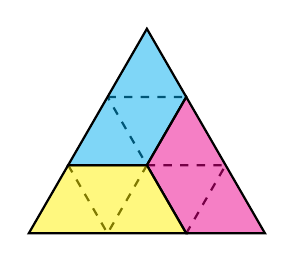
\begin{tikzpicture}
    \draw[thick, dashed]
      (1,0)--(2,0)--(1.5, {-sqrt(3)/2})
      (0,0)--(0.5, {-sqrt(3)/2})--(1,0)--(0.5,{sqrt(3)/2})
      (0.5,{sqrt(3)/2})--(1.5,{sqrt(3)/2});
    \draw[thick, fill=cyan, fill opacity=0.5] (0,0)--(1,{sqrt(3)})--(1.5,{sqrt(3)/2})--(1,0)--cycle;
    \draw[thick, fill=magenta, fill opacity=0.5] (1.5,{sqrt(3)/2})--(2.5,{-sqrt(3)/2})--(1.5,{-sqrt(3)/2})--(1,0)--cycle;
    \draw[thick, fill=yellow, fill opacity=0.5] (-0.5,{-sqrt(3)/2})--(0,0)--(1,0)--(1.5,{-sqrt(3)/2})--cycle;
  \end{tikzpicture}
  \\~\\
  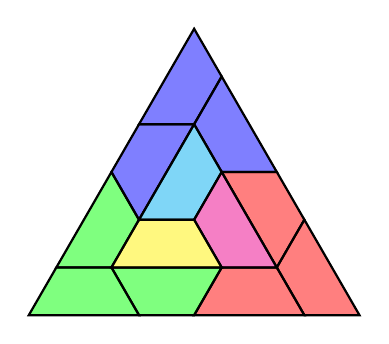
\begin{tikzpicture}[scale=0.7]
    \draw[thick, fill=green, fill opacity=0.5] (0,0)--(1,{sqrt(3)})--(1.5,{sqrt(3)/2})--(1,0)--cycle;
    \draw[thick, fill=blue, fill opacity=0.5] (1,{sqrt(3)})--(1.5,{sqrt(3)/2})--(2.5, {3/2*sqrt(3)})--(1.5, {3/2*sqrt(3)})--cycle;
    \draw[thick, fill=blue, fill opacity=0.5] (1.5,{3/2*sqrt(3)})--(2.5,{5/2*sqrt(3)})--(3,{2*sqrt(3)})--(2.5,{3/2*sqrt(3)})--cycle;
    \draw[thick, fill=blue, fill opacity=0.5] (3,{2*sqrt(3)})--(4,{sqrt(3)})--(3,{sqrt(3)})--(2.5,{3/2*sqrt(3)})--cycle;
    \draw[thick, fill=red, fill opacity=0.5] (4,0)--(3,{sqrt(3)})--(4,{sqrt(3)})--(4.5,{sqrt(3)/2})--cycle;
    \draw[thick, fill=red, fill opacity=0.5] (4,0)--(4.5,{sqrt(3)/2})--(5.5,{-sqrt(3)/2})--(4.5,{-sqrt(3)/2})--cycle;
    \draw[thick, fill=red , fill opacity=0.5] (4.5,{-sqrt(3)/2})--(4,0)--(3,0)--(2.5,{-sqrt(3)/2})--cycle;
    \draw[thick, fill=green, fill opacity=0.5] (2.5,{-sqrt(3)/2})--(3,0)--(1,0)--(1.5,{-sqrt(3)/2})--cycle;
    \draw[thick, fill=green, fill opacity=0.5] (-0.5,{-sqrt(3)/2})--(0,0)--(1,0)--(1.5,{-sqrt(3)/2})--cycle;

    \draw[thick, fill=cyan, fill opacity=0.5] (1.5,{sqrt(3)/2})--(2.5,{3/2*sqrt(3)})--(3,{sqrt(3)})--(2.5,{sqrt(3)/2})--cycle;
    \draw[thick, fill=magenta, fill opacity=0.5] (3,{sqrt(3)})--(4,0)--(3,0)--(2.5,{sqrt(3)/2})--cycle;
    \draw[thick, fill=yellow, fill opacity=0.5] (1,0)--(1.5,{sqrt(3)/2})--(2.5,{sqrt(3)/2})--(3,0)--cycle;
    % \node at (2.5,-1.3) {(primitive)};
  \end{tikzpicture}
  \hspace{0.5cm}
  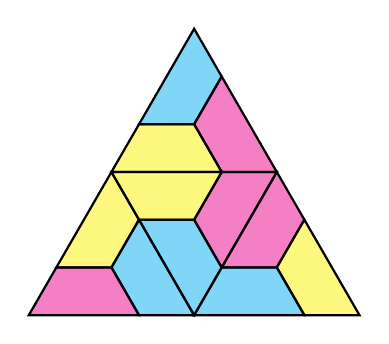
\begin{tikzpicture}[scale=0.7]
    \draw[thick, fill=yellow, fill opacity=0.5] (0,0)--(1,{sqrt(3)})--(1.5,{sqrt(3)/2})--(1,0)--cycle;
    \draw[thick, fill=cyan, fill opacity=0.5] (1.5,{sqrt(3)/2})--(2.5,{-sqrt(3)/2})--(1.5,{-sqrt(3)/2})--(1,0)--cycle;
    \draw[thick, fill=magenta, fill opacity=0.5] (-0.5,{-sqrt(3)/2})--(0,0)--(1,0)--(1.5,{-sqrt(3)/2})--cycle;

    % Lower right
    \draw[thick, fill=magenta, fill opacity=0.5] (3,0)--(4,{sqrt(3)})--(4.5,{sqrt(3)/2})--(4,0)--cycle;
    \draw[thick, fill=yellow, fill opacity=0.5] (4.5,{sqrt(3)/2})--(5.5,{-sqrt(3)/2})--(4.5,{-sqrt(3)/2})--(4,0)--cycle;
    \draw[thick, fill=cyan, fill opacity=0.5] (2.5,{-sqrt(3)/2})--(3,0)--(4,0)--(4.5,{-sqrt(3)/2})--cycle;

    % Upper
    \draw[thick, fill=cyan, fill opacity=0.5] (1.5,{3/2*sqrt(3)})--(2.5,{5/2*sqrt(3)})--(3,{2*sqrt(3)})--(2.5,{3/2*sqrt(3)})--cycle;
    \draw[thick, fill=magenta, fill opacity=0.5] (3,{2*sqrt(3)})--(4,{sqrt(3)})--(3,{sqrt(3)})--(2.5,{3/2*sqrt(3)})--cycle;
    \draw[thick, fill=yellow, fill opacity=0.5] (1,{sqrt(3)})--(1.5,{3/2*sqrt(3)})--(2.5,{3/2*sqrt(3)})--(3,{sqrt(3)})--cycle;

    % Upside down
    \draw[thick, fill=cyan, fill opacity=0.5] (1.5,{1/2*sqrt(3)})--(2.5,{-1/2*sqrt(3)})--(3,0)--(2.5,{1/2*sqrt(3)})--cycle;
    \draw[thick, fill=magenta, fill opacity=0.5] (3,0)--(4,{sqrt(3)})--(3,{sqrt(3)})--(2.5,{1/2*sqrt(3)})--cycle;
    \draw[thick, fill=yellow, fill opacity=0.5] (1,{sqrt(3)})--(1.5,{1/2*sqrt(3)})--(2.5,{1/2*sqrt(3)})--(3,{sqrt(3)})--cycle;
  \end{tikzpicture}
  \hspace{0.5cm}
  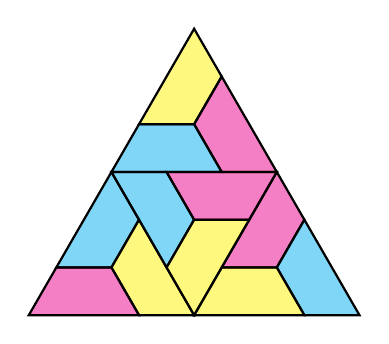
\begin{tikzpicture}[scale=0.7]
    \draw[thick, fill=cyan, fill opacity=0.5] (0,0)--(1,{sqrt(3)})--(1.5,{sqrt(3)/2})--(1,0)--cycle;
    \draw[thick, fill=yellow, fill opacity=0.5] (1.5,{sqrt(3)/2})--(2.5,{-sqrt(3)/2})--(1.5,{-sqrt(3)/2})--(1,0)--cycle;
    \draw[thick, fill=magenta, fill opacity=0.5] (-0.5,{-sqrt(3)/2})--(0,0)--(1,0)--(1.5,{-sqrt(3)/2})--cycle;

    % Lower right
    \draw[thick, fill=magenta, fill opacity=0.5] (3,0)--(4,{sqrt(3)})--(4.5,{sqrt(3)/2})--(4,0)--cycle;
    \draw[thick, fill=cyan, fill opacity=0.5] (4.5,{sqrt(3)/2})--(5.5,{-sqrt(3)/2})--(4.5,{-sqrt(3)/2})--(4,0)--cycle;
    \draw[thick, fill=yellow, fill opacity=0.5] (2.5,{-sqrt(3)/2})--(3,0)--(4,0)--(4.5,{-sqrt(3)/2})--cycle;

    % Upper
    \draw[thick, fill=yellow, fill opacity=0.5] (1.5,{3/2*sqrt(3)})--(2.5,{5/2*sqrt(3)})--(3,{2*sqrt(3)})--(2.5,{3/2*sqrt(3)})--cycle;
    \draw[thick, fill=magenta, fill opacity=0.5] (3,{2*sqrt(3)})--(4,{sqrt(3)})--(3,{sqrt(3)})--(2.5,{3/2*sqrt(3)})--cycle;
    \draw[thick, fill=cyan, fill opacity=0.5] (1,{sqrt(3)})--(1.5,{3/2*sqrt(3)})--(2.5,{3/2*sqrt(3)})--(3,{sqrt(3)})--cycle;

    % Upside down
    \draw[thick, fill=cyan, fill opacity=0.5] (1,{sqrt(3)})--(2,0)--(2.5,{1/2*sqrt(3)})--(2,{sqrt(3)})--cycle;
    \draw[thick, fill=yellow, fill opacity=0.5] (2.5,{-1/2*sqrt(3)})--(3.5,{1/2*sqrt(3)})--(2.5,{1/2*sqrt(3)})--(2,0)--cycle;
    \draw[thick, fill=magenta, fill opacity=0.5] (2,{sqrt(3)})--(2.5,{1/2*sqrt(3)})--(3.5,{1/2*sqrt(3)})--(4,{sqrt(3)})--cycle;
  \end{tikzpicture}


  \caption{
    A equilateral triangle made of $3$-trapezoids.
  }
\end{figure}
\begin{question}
  Can all trapezoids (that are made out of equilateral triangles) be arranged to
  form an equilateral triangle?
\end{question}

\begin{related}
  \item What is the smallest triangle that can be formed this way?
  \item Is there a construction that makes such triangles given some $k$-trapezoid?
  \item How many such tilings exist for a given size trapezoid and triangle?
  \item Can other shapes be tiled (e.g. hexagon, arbitrary trapezoid)?
  \item Does this generalize to square/hexagonal tilings? Multiple dimensions?
\end{related}

\begin{note}
  If $c(n)$ counts the number of distinct minimal covering sets of $n$-ominoes,
  then $c(1) = c(2) = c(3) = 1$, $c(4) = c(5) = 2$, and $c(6) = 14$.
\end{note}

\begin{references}
  \item Problem 85
  \item \url{https://math.stackexchange.com/q/2215781/121988}
\end{references}
\end{document}
